\documentclass[10pt,a4paper,twoside,openany,hidelinks]{book}
\usepackage{maths}
\usepackage{stylish}

\title{Lecture Notes to a course in Algebraic Topology \\ \large{Winter 2018, Technion IIT}}
\author{Lectures by Nir Lazerovich \\ \large Typed by Elad Tzorani}
\date{\today}

\begin{document}
\frontmatter
\frontpage{simplicial_complex}
\tableofcontents
\countlectures
\newpage

\chapter*{Preface}
\addcontentsline{toc}{chapter}{Preface} \markboth{Preface}{}

\section*{Technicalities}
\addcontentsline{toc}{section}{Technicalities} %\markboth{Technicalities}{}

These aren't formal notes related to the course and henceforward there is \emph{absolutely no guarantee} that the recorded material is in correspondence with the course expectations, or that these notes lack any mistakes.\\
In fact, there probably are mistakes in the notes! I would highly appreciate if any comments or corrections were sent to me via email at \href{mailto:tzorani.elad@gmail.com}{tzorani.elad@gmail.com}.\\
Elad Tzorani.

\section*{Course Literature}
\addcontentsline{toc}{section}{Course Literature} %\markboth{Course Literature}{}

The recommended course literature is as follows.
\begin{description}
\item[Hatcher:] Algebraic Topology
\item[Munkres:] Elements of Algebraic Topology
\end{description}

\mainmatter

\chapter{Motivation}

\section{What is Algebraic Topology?}

\subsection{Homotopy groups}

We'd want to study topological spaces, but that is generally a difficult task. For that reason we associate algebraic objects to topological spaces, through which we can study topology algebraically.
Some reasons for associating algebraic objects to topological spaces are as follows.
\begin{enumerate}
\item Distinguishing spaces.
\item Studying properties of spaces.
\end{enumerate}
\begin{example}[application of Algebraic Topology: Brouwer's fixed point theorem]
Let $\DD^n = \set{x \in \RR^n}{\norm{x} \leq 1}$.
Every continuous map $f \colon \DD^n \to \DD^n$ has a fixed point.
I.e. there's $x \in \DD^n$ such that $f(x) = x$.
\end{example}
\begin{definition}
Let $X$ be a topological space and let $A \subseteq X$. A \stress{retraction} is a continuous map $r \colon X \to A$ such that $\eval{r}{A}{} = \mathrm{id}_A$.
\[
\begin{tikzcd}
X \arrow[r, "r"] & A \\
A \arrow[u, "i", hook] \arrow[ru, "\id", swap] &
\end{tikzcd}
\]
\end{definition}
\begin{lemma}
There is no retraction $\DD^n \to \del \DD^n = \SS^{n-1} = \set{x \in \DD^n}{\norm{x}=1}$.
\end{lemma}
We show that the lemma implies Brouwer's fixed point theorem. \\
\begin{proof}
Assume $\forall x \in \DD^n \colon f(x) \neq x$.
Define $F(x)$ to be the point on $\SS^{n-1}$ intersecting the ray from $f(x)$ to $x$. See figure \ref{retraction_lemma}.
This is continuous (\textbf{check this!}), and hence a retraction, contradicting the lemma.
\begin{figure}[h!]
\begin{center}
\caption{Retraction from the disk to the sphere.}
\label{retraction_lemma}
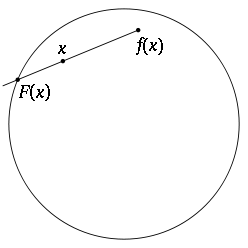
\includegraphics[scale=0.7]{sources/retraction_lemma}
\end{center}
\end{figure}
\end{proof}
We shall now prove the lemma.
\begin{proof}[of the lemma]
\begin{description}
\item[$n=1$:]
Define $\pi_0\prs{X} \ceq \set{\text{path connected componenets of $X$}}$.
A map $f \colon X \to Y$ which is continuous defines a map $\pi_0\prs{f} = f_{*} \colon \pi_0\prs{X} \to \pi_0\prs{Y}$ by $\brs{x} \mapsto \brs{f(x)}$ (this is well defined).
We observe that $\id_{*} = \id_{\pi_0\prs{X}}$.
Also, if $f \colon X \to Y$ and $g \colon Y \to Z$ then $\prs{g \circ f}_{*} = g_{*} f_{*}$.
Assume $r \colon \DD^1 \to \DD^1 = \SS^0$ is a retraction. We apply $\pi_0$ to
\[\
\begin{tikzcd}
\DD^1 \arrow[r, "r"] & \SS^0 \\
\SS^0 \arrow[u, "i", hook] \arrow[ru, "\id", swap] &
\end{tikzcd}
\]
and get the following diagram.
\[
\begin{tikzcd}
\pi_0\prs{\DD^1} \arrow[r, "r_*"] & \pi_0\prs{\SS^0} \\
\pi_0\prs{\SS^0} \arrow[u, "i_*"] \arrow[ru, "\id_* = \id", swap] &
\end{tikzcd}
\]

Now $\pi_0 \prs{\DD^1} = \text{singleton}$
and $\pi_0\prs{\SS^0} = \text{$2$ elements}$
contradicting the diagram.
\item[$n=2$:]
Let $\pi_1\prs{X,x_0}$ be the fundamental group. That is \[\pi_1\prs{X,x_0} = \pi_0\prs{\text{loops in $X$ that start and end in $x_0$}}\text{.}\]
Let $f \colon \prs{X, x_0} \to \prs{Y, y_0}$ be continuous (with $f\prs{x_0} = y_0$). This defines $\pi_1\prs{f} = f_{*} \colon \pi_1\prs{X,x_0} \to \pi_1\prs{Y,y_0}$.
It can be checked (and is showed in another topology course) that $\pi_1\prs{\DD^2, x} \cong 1$, and that $\pi_1\prs{\SS^1, x} \cong \Z$.
We get the following diagram, which gives a contradiction.

\[
\begin{tikzcd}
\pi_1\prs{\DD^2} \cong 1 \arrow[r, "r_*"] & \pi_1\prs{\SS^1} \cong \ZZ \\
\pi_1\prs{\SS^1} \cong \ZZ \arrow[u, "i_*"] \arrow[ru, "\id_* = \id", swap] &
\end{tikzcd}
\]

\end{description}
\end{proof}
We'd want to iterate such a construction by looking at loop spaces of loop spaces.\\
\begin{definition}
\[\pi_n = \pi_0 \prs{\text{loop of} \prs{\text{loop of} \ldots \prs{X, x_0} \tilde{x}_0, \ldots}}\]
\end{definition}
For $n \geq 1$, $\pi_n$ is a group. $\pi_1$ is a group with the operation of concatenation, and we can view $\pi_n$ as $\pi_1$ of some space, if $n \geq 1$. \\
We don't really like this inductive definition of $\pi_n$, so we'd like to give another definition. We can view $\pi_1$ as homotopy classes of $\prs{\SS^1, *} \to \prs{X, x_0}$. We'd like to generalise upon that idea. \\
\begin{definition}
$\pi_n$ is the group of homotopy classes of maps $\prs{\SS^n, *} \to \prs{X, x_0}$. We can view $\SS^n$ as $\quot{I^n}{\del I^n}$, and the group action of $\pi_n$ is given by gluing the spheres at the identified boundary of $\I^n$. It can be checked that $\pi_n$ is abelian for $n \geq 2$.
\end{definition}

\subsection{Homology and cohomology of topological spaces}
Homotopy groups are relatively difficult to compute. We'd want to introduce another algebraic object associate to topological spaces, $\tilde{H}_n$, which we shall see satisfies $\tilde{H}_n\prs{\SS^k} = \fcases{ 0 & n\neq k \\ \Z & n = k}$. We'll use this structure to prove Brouwer's theorem. \\
We define $H_0\prs{X} = \bigoplus_{\pi_0} \Z$ \stress{the zero'th homology group}, and similarly  $H_1\prs{X} = \pi_1\prs{X,x_0}^{\mathrm{ab}}$ \stress{the first homology group}.
\backmatter
\end{document}